\section{Analyse des Marktes}


\subsection{Zielgruppe und potenzielle Kunden}
SemLit richtet sich auf alle, die in der wissenschaftliche Bereich tätig sind. Semlit ist eine Dienstleistung, die Wissenschaftler in unterschiedliche Bereichen der Forschung und Entwicklung unterstützen wird. Die Konsumenten könnten in drei Gruppen gegliedert werden:
\begin{itemize}
\item Private Personen (Studenten und Wissenschaftler)

\item Wissenschaftliche Einrichtungen (Universitäten, Forschungszentren)

\item Unternehmen (Forschungs- und Entwicklungsabteilungen)
\end{itemize}


\subsection{Marktsituation}
Die Marktanalyse wird auf Basis von UNESCO Science Report 2010 durchgeführt. Dieser Bericht stellt wichtige Daten über die Große, potenzielle Entwicklungsrichtungen und Wachstum der Wissenschaft zusammen.\\
Die Endnutzer der SemLit sind Wissenschaftler, deswegen  die potenzielle Entwicklungsrichtungen des Marktes aus Daten über Anzahl der Wissenschaftler in der Welt abgeleitet werden können. In der Bericht von UNESCO kann man die Daten für 2002 und 2007 Jahre finden und Wachstum schätzen.\\
Wie kann man aus Abbildung \ref{fig:fig1} sehen, der gesamte Anzahl der Wissenschaftler in der Welt hat sich von 5 810 700 auf 7 209 700 Wissenschaftler erhöht, was entspicht ein Wachstum um ca. 24\% in 5 Jahren. Die größte Anteil sind die Wissenschaftler aus entwickelten Länder, aber Entwicklungsländer zeigen größere Wachstumspotenzial in Höhe von ca. 55,5 \% in 5 Jahre, gegen ca. 10,6\% Wachstum für entwickelten Länder.\\
\begin{figure}[h!]
\centering
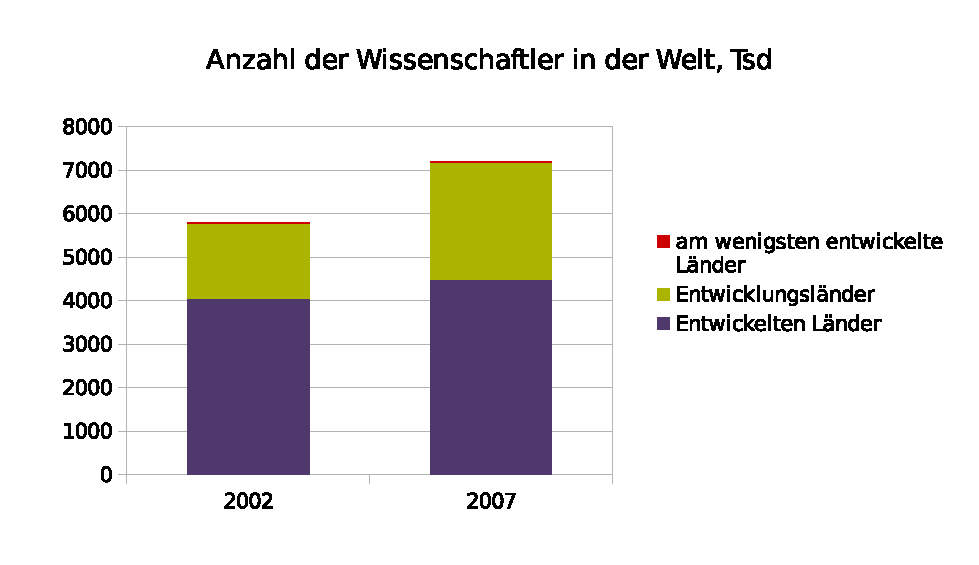
\includegraphics[width=0.8\textwidth]{fig1}
\caption{Anzahl der Wissenschaftler in der Welt, UNESCO 2010}
\label{fig:fig1}
\end{figure}
Andere Daten, die oben genannte Tendenz bestätigen, sind die Anzahl der Publikationen in der Welt. In 6 Jahre hat sich die Anzahl der Publikationen von 733305 auf 986099 erhöht, was ca. 34,5\% der Erhöhung entspricht. Die größte Anzahl gehört zur entwickelten Länder, aber Entwicklungsländer zeigen signifikante 105,9\% Wachstum (Abbildung \ref{fig:fig2})\\
\begin{figure}[h!]
\centering
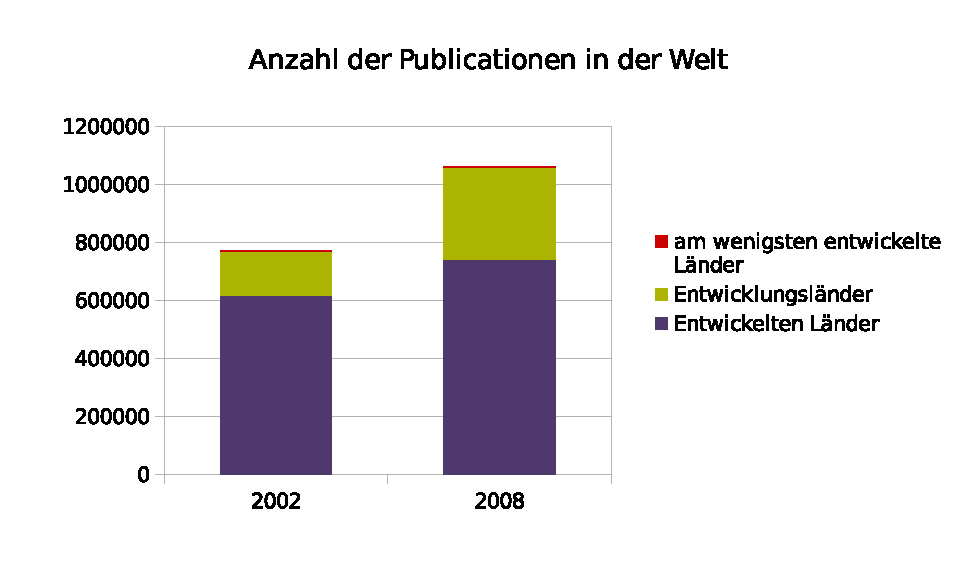
\includegraphics[width=0.8\textwidth]{fig2}
\caption{Anzahl der Publikationen in der Welt, UNESCO 2010}
\label{fig:fig2}
\end{figure}
Auf Grund dieser Daten, kann man feststellen, dass  wichtige Märkte sich in entwickelte Länder befinden. Die Entwicklungsländer zeigen aber riesige Wachstumspotenzial und sollte auch berücksichtigen werden. 
Als Zusammenfassung kann man sagen, dass die Markt der Potenzielle Kunden in letzte Jahren eine gute Wachstum gezeigt hat und eine gute Aufsicht auf weitere Entwicklung besitzt.

\subsection{Auswahl der regionale Märkte}
Auswahl von regionale Märkte ist wichtige Teil der Marketingstrategie. Konzentration auf nur begrenzte Liste der regionale Märkte lasst die  regionale Eigenschaften berücksichtigen und möglichst beste Dienstleistung anzubieten. Enge Zusammenarbeit auf regionale Markt und Partnerprogrammen sollten Erfolg der Absatz unterstützen und neue Richtungen in Entwicklung darstellen.\\
Um richtige regionale Märkte auszuwählen, wird es nur die Länder ausgewählt, die maximale Anzahl der Wissenschaftler haben, da die Wissenschaftler die Endnutzer der SemLit sind. \\
Das Auswahl der Länder erfolgt mit Hilfe der Angaben von UNESCO 2010 über die Anzahl der Wissenschaftler in jedes Land. Es wird nur die Länder ausgewählt, die zusammen ca. 70\% von der gesamte Anzahl alle Wissenschaftler in der Welt bauen. Die Zusammenfassung der Entwicklung der Anzahl der Wissenschaftler ist in der Tabelle \ref{tab:ABC} dargestellt.\\
Wie kann man aus Tabelle \ref{tab:ABC} sehen, acht ausgewählte Länder bauen ca. 70\% von alle Wissenschaftler in der Welt. Viele von denen zeigen auch signifikante Erhöhung um mehr als 50\% in 5 Jahre. Dieser Länder sind China und Südkorea.
\begin{table}[h!]
  \centering
  \begin{tabular}{|l|r|r|r|r|r|}\hline
  \textbf{Land} & \multicolumn{4}{ c| }{\textbf{Anzahl der Wissenschaftler, Tsd.}} & \textbf{Wachstum}\\
  & 2002 & \% gesamt & 2007 & \% gesamt & \\ \hline
Welt & 5810.7 & 100.00\% & 7209.7 & 100.00\% & 24.08\% \\ \hline
Vereinigte Staaten & 1342.5 & 23.10\% & 1425.6 & 19.77\% & 6.19\% \\
China & 810.5 & 13.95\% & 1423.4 & 19.74\% & 75.62\% \\
Japan & 646.5 & 11.13\% & 710 & 9.85\% & 9.82\% \\
Russische Föderation & 491.9 & 8.47\% & 469.1 & 6.51\% & -4.64\% \\
Deutschland & 265.8 & 4.57\% & 290.9 & 4.03\% & 9.44\% \\
Vereinigtes Königreich & 198.2 & 3.41\% & 254.6 & 3.53\% & 28.46\% \\
Südkorea & 141.9 & 2.44\% & 221.9 & 3.08\% & 56.38\% \\
Frankreich & 186.4 & 3.21\% & 215.8 & 2.99\% & 15.77\% \\
Kanada & 116 & 2.00\% & 139 & 1.93\% & 19.83 \% \\ \hline
Alle ausgewählte Länder & 4199.7 & 72.28\% & 5150.3 & 71.44\% & 22.63\% \\ \hline
  \end{tabular}
  \caption{Länder mit größte Anteil der Wissenschaftler, basiert auf Daten von UNESCO 2010}
  \label{tab:ABC}
\end{table}

Für alle ausgewählte Länder wird andere wichtige Parameter geschätzt, Bruttoinlandsausgaben für Forschung und Entwicklung (GERD) pro ein Wissenschaftler. Dieser Parameter könnte zeigen, wie viel Geld in der Forschung und Entwicklung investiert wird. Je mehr dieser Zahl ist, desto mehr ist die Wahrscheinlichkeit, dass Wissenschaftler das Geld nicht nur für reine Forschung, sonder auch für Dienstleistung, die dieser Forschung erleichtern könnten, zahlen werden. In Tabelle \ref{tab:ABC2} sind die Angaben zum Entwicklung der Bruttoinlandsausgaben für Forschung und Entwicklung pro ein Wissenschaftler präsentiert. Wie kann man aus Tabelle \ref{tab:ABC2} sehen, entwickelte Länder investieren sehr viel Geld in Forschung und Entwicklung, was als gute Möglichkeit für Absatz sprechen kann. 
\begin{table}[h!]
  \centering
  \begin{tabular}{|l|p{3cm}|p{3cm}|r|}\hline
  \textbf{Land} & \multicolumn{2}{ r| }{\textbf{GERD pro Wissenschaftler, \$ Tsd.}} & \textbf{Wachstum} \\
  & 2002 & 2007 & \\ \hline
Deutschland & 213.1& 248.4 & 16.56\% \\
Vereinigte Staaten & 206.4 & 243.9 & 18.17\% \\
Japan & 167.3 & 208.4 & 24.57\% \\
Frankreich & 204.7 & 196.1 & -4.20\% \\
Südkorea & 158.6 & 186.3 & 17.47\% \\
Kanada & 165 & 170.7 & 3.45\% \\
Vereinigtes Königreich & 154.6 & 152.2 & -1.55\% \\
China & 48.4 & 72 & 48.76\% \\
Russische Föderation & 32.4 & 50.1 & 54.63\% \\ \hline
  \end{tabular}
  \caption{Bruttoinlandsausgaben für Forschung und Entwicklung (GERD) pro ein Wissenschaftler, basiert auf Daten von UNESCO 2010}
  \label{tab:ABC2}
\end{table} 



\subsection{Schätzung der Marktvolumen}
Schätzung der Marktvolumen ist für Bereich Wissenschaft schwierig, da genauer Daten über die Anzahl und Budget nicht die Realität abbilden können. Deswegen werden dieser Daten grob aus vorhandene Daten abgeleitet. Zuerst wird die gesamt Anzahl der Wissenschaftler und Bruttoinlandsausgaben für Forschung und Entwicklung in ausgewählte regionale Märkte berechnet. Dann Anzahl von alle Publikationen und Anzahl von Publikationen in Bereich von Ingenieurwesen und Technologie, die in dieser Länder publiziert worden. Aus resultierte Daten von Anzahl der Publikationen, könnte ein Verhältnis-Koeffizient berechnet werden, die grobe Schätzung über die Anteil von Ingenieurwesen und Technologie in gesamte Wissenschaftliche Tätigkeit geben kann. Andere Koeffizienten, die wichtig sein könnten, sind Verhältnis von Anzahl der Wissenschaftler / Anzahl der alle Publikationen und Verhältnis von Bruttoinlandsausgaben für Forschung und Entwicklung / Anzahl der alle Publikationen. Dieser Koeffizienten zeigen, dass durchschnittlich 7 Wissenschaftler auf eine Publikation arbeiten und durchschnittliche Bruttoinlandsausgaben für eine Publikation ca. 1137,8 Tsd. von PPP\$ ist.
\begin{table}[h!]
  \centering
  \begin{tabular}{|l|l|}\hline
   \textbf{Parameter} &  \textbf{Wert} \\ \hline
  Anzahl der Wissenschaftler & 5150300 \\ \hline
  Bruttoinlandsausgaben für Forschung und Entwicklung & 865,5 Mrd. PPP\$ \\ \hline
  Anzahl der alle Publikationen & 760671 \\ \hline
  Anzahl der Publikationen in Ingenieurwesen & 101351
 \\
  und Technologie& \\ \hline
  Verhältnis (Publikationen in Ing.\& Tech. / alle Publikationen) & 13,3\% \\ \hline
  Verhältnis (Anzahl der Wissenschaftler / Anzahl der & ca. 7 \\
  alle Publikationen ) & \\ \hline
  Verhältnis (Bruttoinlandsausgaben für Forschung & 1137,8 Tsd. PPP\$\\
  und Entwicklung / Anzahl der alle Publikationen) & \\ \hline
  \end{tabular}
  \caption{Angaben zur Märkte, basiert auf Daten von UNESCO 2010}
  \label{tab:ABC3}
\end{table}
 

\subsection{Wettbewerber}
Die wesentliche Wettbewerber, die in der Feld der Akademische Suche sind Suchmaschinen. Normalweise, Suchmaschinen bieten keine Zugang zum Volltext, sondern zur Abstrakt und Referenzen. Wichtige Suchmaschine sind in Tabelle \ref{tab:wettSuch} zusammengefasst.
\begin{table}[h!]
  \centering
  \begin{tabular}{|l|l|l|l|}\hline
   \textbf{Name} &  \textbf{Suchverfahren} &  \textbf{Suchbereiche} &   \textbf{Zugang} \\ \hline
BASE - Bielefeld Academic  & Fast Search \& & Interdisziplinär & Kostenfrei \\
Search Engine & Transfer  & & \\ \hline
 Google Scholar & Eigene & Interdisziplinär & Kostenfrei\\\hline
 Microsoft Academic & Vertikale & Informatik & Kostenfrei \\
 Search & Suchmaschine & & \\ \hline
 CiteSeer & Eigene & Informatik & Kostenfrei \\ \hline
  \end{tabular}
  \caption{Wichtige Suchmaschine}
  \label{tab:wettSuch}
\end{table} 
 
Zur zweite Gruppe gehören Datenbanken. Sie stellen nicht nur Suche in Abstrakt und Referenzen, sondern auch Zugang zur Volltexte. Normalweise, Suche und Zugang zum Abstrakt sind kostenfrei. Um Zugang zum Volltext zu bekommen, soll man eine Abonnement kaufen. Wichtige Datenbanken sind in der Tabelle \ref{tab:wettDaten} gelistet. 
\begin{table}[h!]
  \centering
  \begin{tabular}{|l|l|l|l|}\hline
  \textbf{Name} &  \textbf{Suchbereiche} &  \textbf{Zugang} &  \textbf{Anbieter} \\ \hline
 SpringerLink & Interdisziplinar & Abonnement & Springer\\ \hline
 Academic Search & Interdisziplinar & Abonnement & EBSCO Publishing\\ \hline
 IEEE Xplore & Informatik \& & Abonnement & IEEE\\ 
 & Elektrotechnik & & \\ \hline
 Scopus & Interdisziplinar & Abonnement & Elsevier\\ \hline
 Web of Science & Interdisziplinar & Abonnement & Thomson ISI \\ \hline
  \end{tabular} 
  \caption{Wichtige Datenbanken}
  \label{tab:wettDaten}
\end{table} 


\subsection{Alleinstellungsmerkmal und Kundennutzen}
Der wesentliche Unterschied zwischen schon existierende Angebote auf Markt und SemLit ist semantische Suche, Verwaltung von Publikationen, Self-Learning Algorithmus, um neue relevante Publikationen zu finden. Auf eine Seite SemLit stellt ein Dienstleistung wie Suchmaschinen auf andere Seite gibt es eine Möglichkeit auf bevorzugte Datenbanken zuzugreifen.\\
SemLit ist sehr flexibel bei Kundennutzung.Wenn die Kunden schon existierende Abonnement für eine der Datenbanken haben, SemLit als eine erweiterte Suchmaschine genutzt werden kann. D.h. Kunden können eine glatte Übergang von vorhandene Lösung zur SemLit durch führen oder SemLit als Erweiterung nutzen. 


